%!TEX root = final_report.tex

\subsection{Unit tests on synthetic datasets}
We tested our implementation on simulated data sets to check its correctness. We generated 4 test sets in the 3-dimensional space and 3 test cases in the 4-dimensional space. Figure \ref{fig: testcases} show a visualization of our 3-dimensional test cases. For simplicity, the range on each axis is set to be $[0, 20]$. In test set 1, there is just a box in the middle of the space. In test set 2, there is one box floating in the middle of the space as well as four smaller boxes on the other side of the space. The smaller boxes, however, should be able to be identified as 1 dense sub-tensor, since the Dcube algorithm is scanning for subsets, rather than continuous ranges, of unique values associated with high density (though definition of density could vary) on each dimension. The four smaller boxes can be expressed the cartesian product of one subset of values along each dimension, therefore they should be identified in the same dense block. In test set 3, we have 3 boxes of various sizes next to each other. A correct implementation should be able to identify the 3 boxes separately. In test set 4, we have  3 boxes alone the spacial diagonal of the space. We expect the algorithm to identify all three boxes easily.

\begin{figure}[h]
\centering 
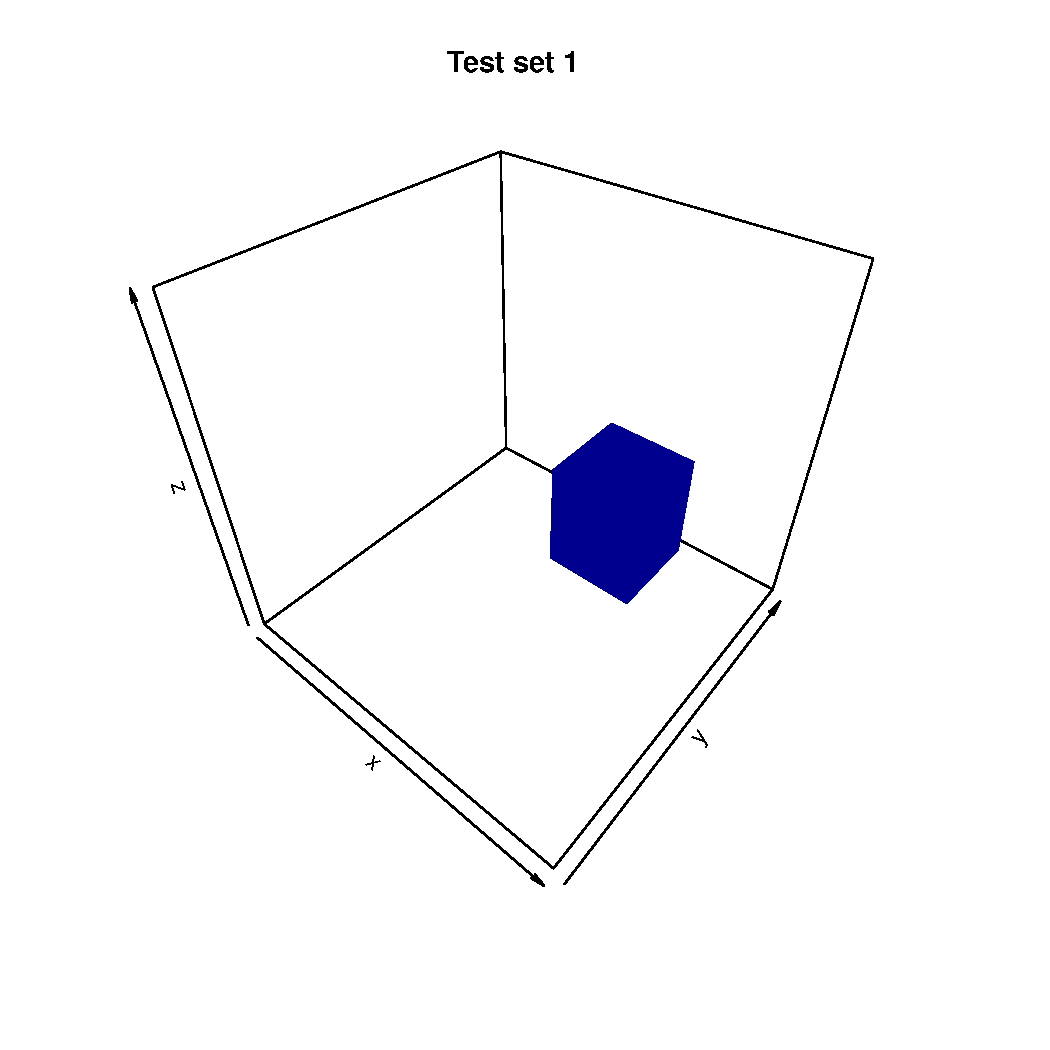
\includegraphics[width=.35\columnwidth]{plots/TS1.pdf} 
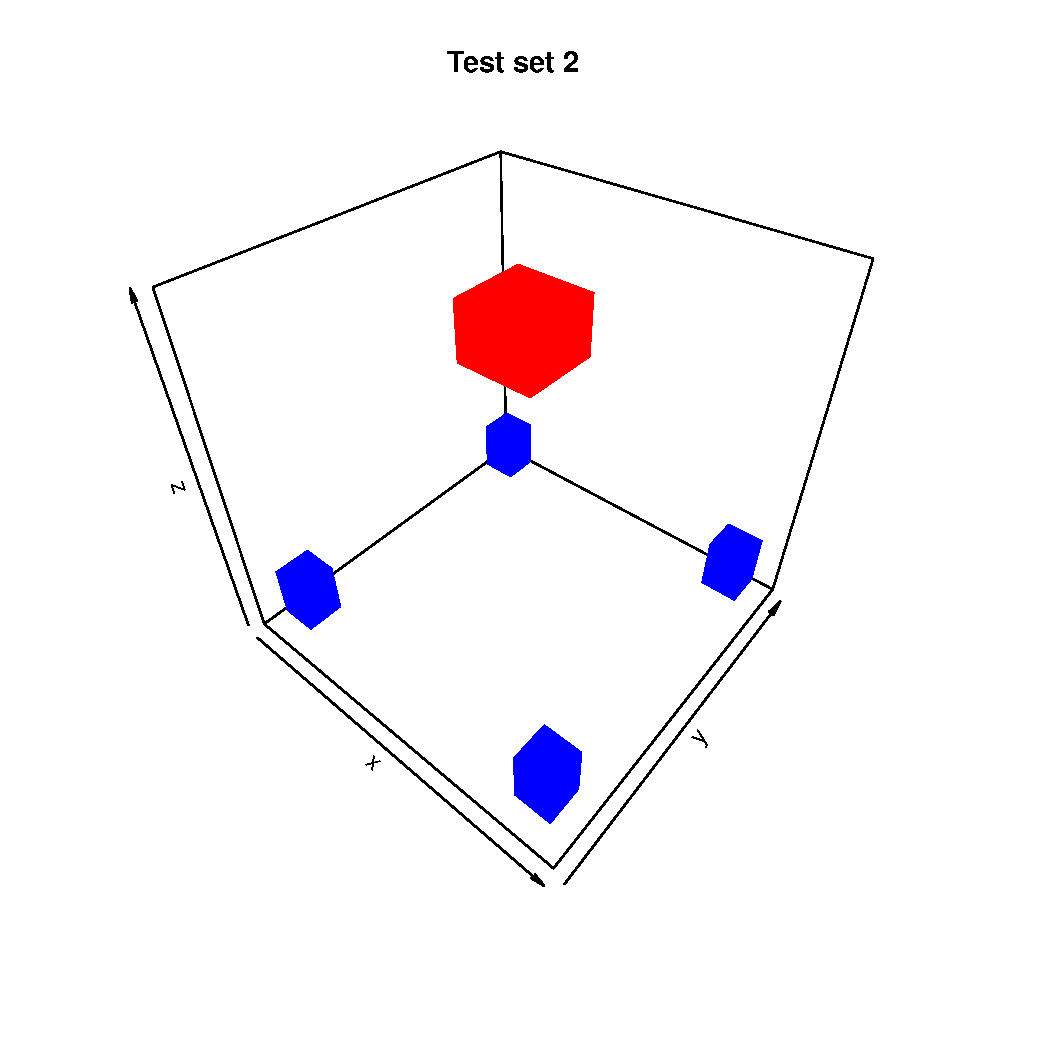
\includegraphics[width=.35\columnwidth]{plots/TS2.pdf} 
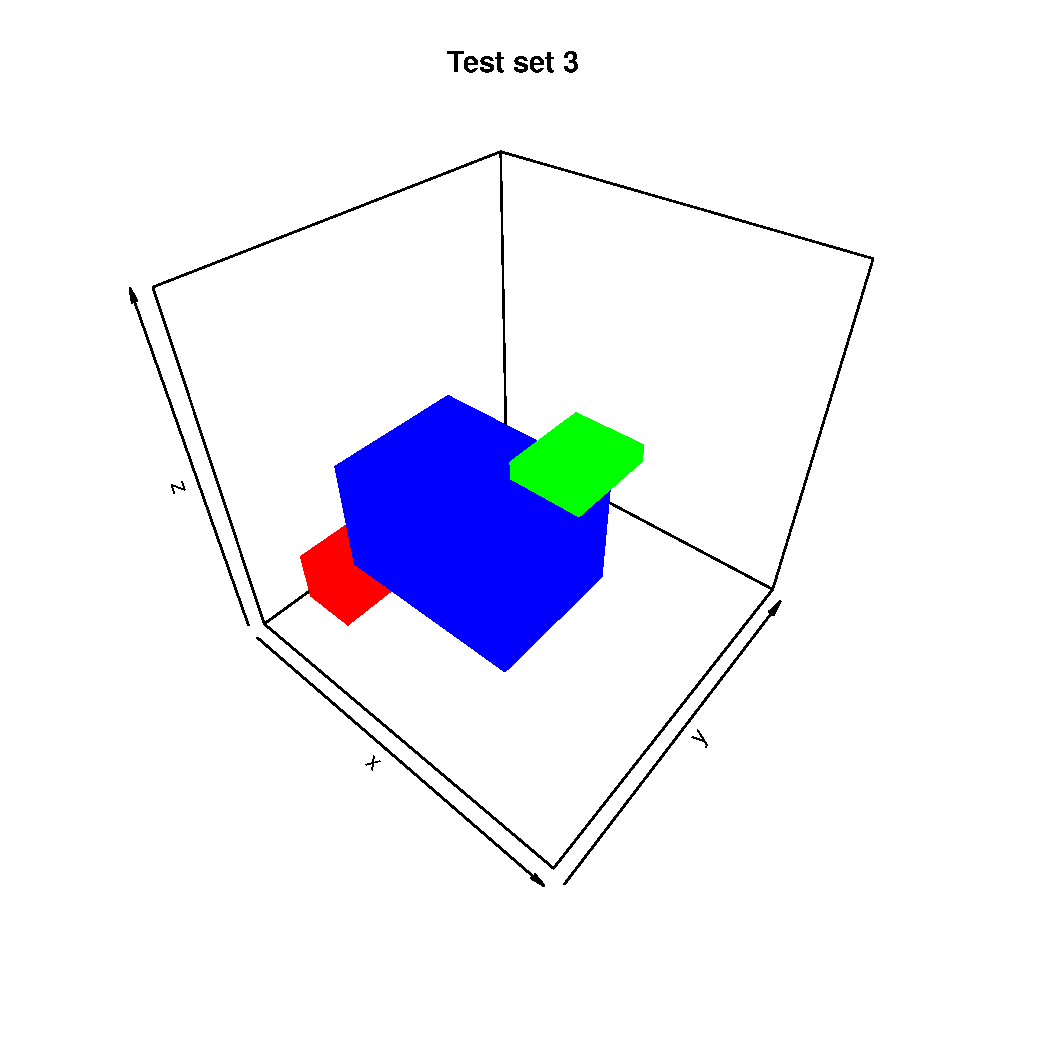
\includegraphics[width=.35\columnwidth]{plots/TS3.pdf} 
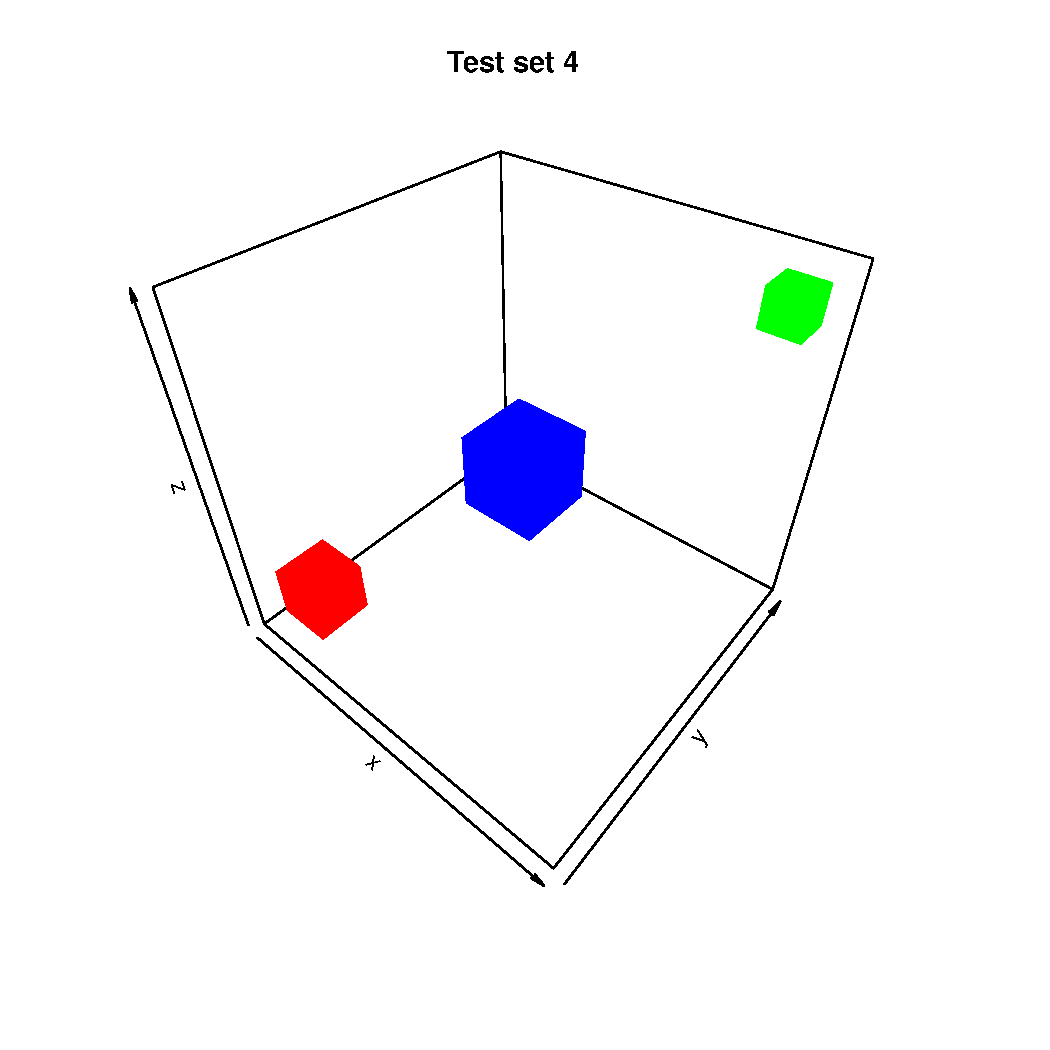
\includegraphics[width=.35\columnwidth]{plots/TS4.pdf} 
\caption{True blocks in test data sets. }
\label{fig: testcases}
\end{figure}

\begin{table}[h]
\centering
\caption{Summary of unit test results in the 3-dimensional space}
\label{table: test3d}
\begin{tabular}{|r|r|r|r|r|r|r|}
\hline
\multicolumn{1}{|c|}{\multirow{2}{*}{\begin{tabular}[c]{@{}c@{}}Dimensionality Selection Policy\\ Density Measure\end{tabular}}} & \multicolumn{3}{c|}{Maximum Density First}                                                  & \multicolumn{3}{c|}{Maximum Cardinality First}                                              \\ \cline{2-7} 
\multicolumn{1}{|c|}{}                                                                                                           & \multicolumn{1}{c|}{Dataset} & \multicolumn{1}{c|}{Precision} & \multicolumn{1}{c|}{Recall} & \multicolumn{1}{c|}{Dataset} & \multicolumn{1}{c|}{Precision} & \multicolumn{1}{c|}{Recall} \\ \hline
\multirow{4}{*}{Arithmatic Average Degree}                                                                                       & Test set 1                   & 1.0                            & 1.0                         & Test set 1                   & 1.0                            & 1.0                         \\ \cline{2-7} 
                                                                                                                                 & Test set 2                   & 1.0                            & 1.0                         & Test set 2                   & 1.0                            & 1.0                         \\ \cline{2-7} 
                                                                                                                                 & Test set 3                   & 1.0                            & 0.978                       & Test set 3                   & 1.0                            & 1.0                         \\ \cline{2-7} 
                                                                                                                                 & Test set 4                   & 1.0                            & 0.922                       & Test set 4                   & 1.0                            & 0.922                       \\ \hline
\multirow{4}{*}{Geometric Average Degree}                                                                                        & Test set 1                   & 1.0                            & 1.0                         & Test set 1                   & 1.0                            & 1.0                         \\ \cline{2-7} 
                                                                                                                                 & Test set 2                   & 1.0                            & 1.0                         & Test set 2                   & 1.0                            & 1.0                         \\ \cline{2-7} 
                                                                                                                                 & Test set 3                   & 1.0                            & 0.978                       & Test set 3                   & 1.0                            & 1.0                         \\ \cline{2-7} 
                                                                                                                                 & Test set 4                   & 1.0                            & 0.922                       & Test set 4                   & 1.0                            & 0.922                       \\ \hline
\multirow{4}{*}{Suspiciousness}                                                                                                  & Test set 1                   & 1.0                            & 1.0                         & Test set 1                   & 1.0                            & 1.0                         \\ \cline{2-7} 
                                                                                                                                 & Test set 2                   & 1.0                            & 1.0                         & Test set 2                   & 1.0                            & 1.0                         \\ \cline{2-7} 
                                                                                                                                 & Test set 3                   & 1.0                            & 1.0                         & Test set 3                   & 1.0                            & 1.0                         \\ \cline{2-7} 
                                                                                                                                 & Test set 4                   & 1.0                            & 0.922                       & Test set 4                   & 1.0                            & 0.922                       \\ \hline
\end{tabular}
\end{table}

\begin{table}[h]
\centering
\caption{Summary of unit tests in the 4-dimensional space}
\label{table: test4d}
\begin{tabular}{|r|r|r|r|r|r|r|}
\hline
\multicolumn{1}{|c|}{\multirow{2}{*}{\begin{tabular}[c]{@{}c@{}}Dimensionality Selection Policy\\ Density Measure\end{tabular}}} & \multicolumn{3}{c|}{Maximum Density First}                                                  & \multicolumn{3}{c|}{Maximum Cardinality First}                                              \\ \cline{2-7} 
\multicolumn{1}{|c|}{}                                                                                                           & \multicolumn{1}{c|}{Dataset} & \multicolumn{1}{c|}{Precision} & \multicolumn{1}{c|}{Recall} & \multicolumn{1}{c|}{Dataset} & \multicolumn{1}{c|}{Precision} & \multicolumn{1}{c|}{Recall} \\ \hline
\multirow{3}{*}{Arithmatic Average Degree}                                                                                       & Test set 1                   & 1.0                            & 1.0                         & Test set 1                   & 1.0                            & 1.0                         \\ \cline{2-7} 
                                                                                                                                 & Test set 2                   & 1.0                            & 0.989                       & Test set 2                   & 1.0                            & 0.989                       \\ \cline{2-7} 
                                                                                                                                 & Test set 3                   & 1.0                            & 0.995                       & Test set 3                   & 1.0                            & 0.995                       \\ \hline
\multirow{3}{*}{Geometric Average Degree}                                                                                        & Test set 1                   & 1.0                            & 1.0                         & Test set 1                   & 1.0                            & 1.0                         \\ \cline{2-7} 
                                                                                                                                 & Test set 2                   & 1.0                            & 0.989                       & Test set 2                   & 1.0                            & 0.989                       \\ \cline{2-7} 
                                                                                                                                 & Test set 3                   & 1.0                            & 0.995                       & Test set 3                   & 1.0                            & 0.995                       \\ \hline
\multirow{3}{*}{Suspiciousness}                                                                                                  & Test set 1                   & 1.0                            & 1.0                         & Test set 1                   & 1.0                            & 1.0                         \\ \cline{2-7} 
                                                                                                                                 & Test set 2                   & 1.0                            & 0.989                       & Test set 2                   & 1.0                            & 0.989                       \\ \cline{2-7} 
                                                                                                                                 & Test set 3                   & 1.0                            & 0.995                       & Test set 3                   & 1.0                            & 0.995                       \\ \hline
\end{tabular}
\end{table}
We summarize the tests based on the above described test sets in Table \ref{table: test3d} and Table \ref{table: test4d}. Given each data set, the output of Dcube algorithm is $k$ blocks. The intersection of the real blocks with positive mass and the $k$ identified blocks can be seen as the true positive results. The entries with positive mass that are not identified by the algorithm can be seen as false negatives, and the entries identified by the algorithm, which have zero mass, are seen as false positives. The precision and recall rates in the following table are calculated using the following formulas.

$$\text{Precision} = \frac{\text{True Positive}}{\text{True Positive + False Positive}}$$
$$\text{Recall} = \frac{\text{True Positive}}{\text{True Positive + False Negative}}$$

As can be seen from Table \ref{table: test3d} and Table \ref{table: test4d}, our current method achieves very high precision and recall score. The majority of blocks are correctly identified, and very little false positive identifications were made.

\subsection{Evaluation}
As is required, we applied the D-cube algorithm on both the DARPA TCP Dump dataset and the Airforce TCP Dump dataset. We used the arithmetic density measure and maximum density policy.

\subsubsection{Top 5 blocks}
We summarize the basic information of the top 5 blocks detected in each dataset in Table \ref{table: k5_2}.

\begin{table}[htbp]
\centering
\caption{Summary of the first 5 blocks on DARPA and Airforce attack dataset}
\label{table: k5_2}
\begin{tabular}{rrrrr}
\hline
Dataset                                                                                    & Order                  & Volume & Mass   & Density  \\ \hline
\multirow{5}{*}{DARPA}                                                                     & \multicolumn{1}{r|}{1} & 94     & 278K   & 16697.28 \\
                                                                                           & \multicolumn{1}{r|}{2} & 2832   & 688K   & 16005.70 \\
                                                                                           & \multicolumn{1}{r|}{3} & 88     & 230K   & 14688.77 \\
                                                                                           & \multicolumn{1}{r|}{4} & 5      & 26K    & 11301.86 \\
                                                                                           & \multicolumn{1}{r|}{5} & 36     & 77K    & 11060.71 \\ \hline
\multirow{5}{*}{Airforce}                                                                  & \multicolumn{1}{r|}{1} & 1      & 1.93M  & 1.93M    \\
                                                                                           & \multicolumn{1}{r|}{2} & 8      & 2.53M  & 1.77M    \\
                                                                                           & \multicolumn{1}{r|}{3} & 131K   & 554K   & 41.7K    \\
                                                                                           & \multicolumn{1}{r|}{4} & 3.71M  & 493K   & 27.2K    \\
                                                                                           & \multicolumn{1}{r|}{5} & 1.4K   & 168.9K & 19K      \\ \hline
\end{tabular}
\end{table}


\subsubsection{ROC curves}

Here, we defined each entry in the dataset labeled as positive as a positive entry. If that entry is identified at a certain stage of the algorithm, then it is regarded as a true positive, otherwise it is regarded as a false negative. Left half of Figure \ref{fig: roc} shows the ROC curve of applying D-cube algorithm on the DARPA TCP Dump dataset with $k = 1, \cdots, 20$. The right half of Figure \ref{fig: roc} similarly shows the ROC curve of D-cube on Airforce TCP Dump dataset. 

\begin{figure}[htbp]
\centering 
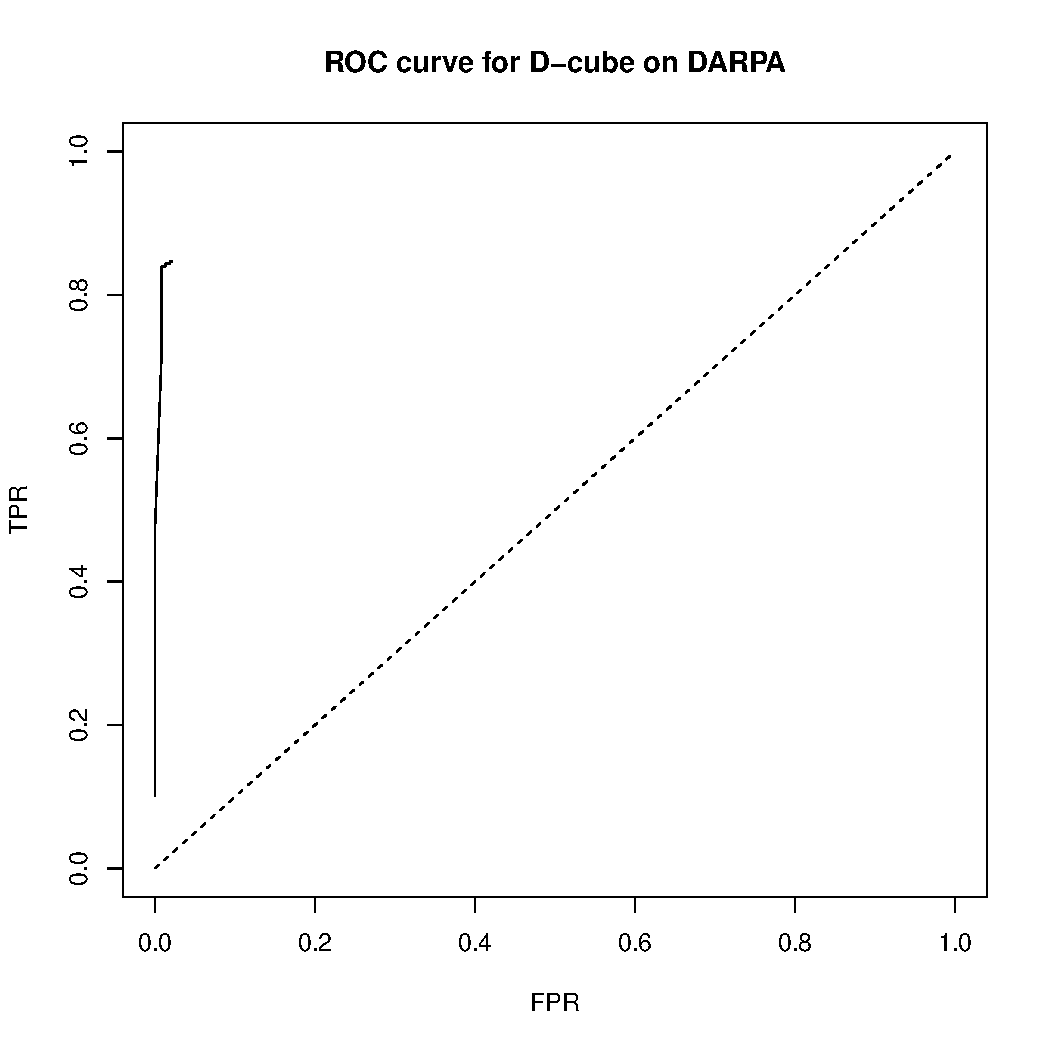
\includegraphics[width=.45\columnwidth]{plots/darpa_ROC.pdf} 
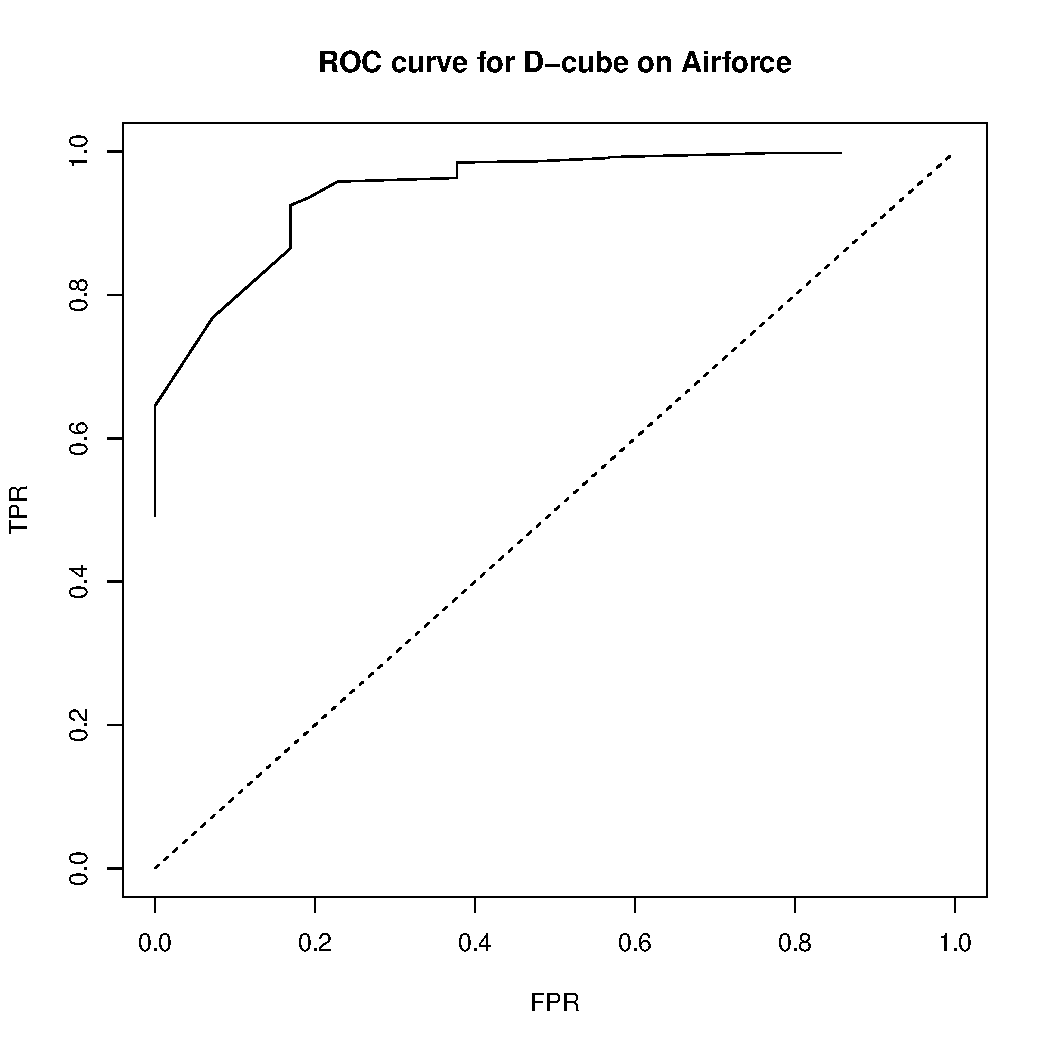
\includegraphics[width=.45\columnwidth]{plots/airforce_ROC.pdf} 
\caption{The ROC curve for $k = 1, \cdots, 20$ by applying the D-cube algorithm on the DARPA TCP Dump dataset (left) and Airforce TCP Dump dataset (right). }
\label{fig: roc}
\end{figure}



%Here, we illustrate the results on DARPA data in Table \ref{table: darpa}, where the timestamps are bucketized by days, and the number of blocks is specified to be $K=1$ due to limited time. We point out that this bucketization by day gives a  very coarse resolution -- all the hours in the entire day are treated as a whole, which will be entirely picked up by a dense block or entirely missed. In addition, when computing the precision and recall rates, the true labels are also bucketized by days: if there is one positive entry in a day, we treat the day as positive as a whole. This is again a rough measurement. Therefore, the current  precision and recall rates are not very high.  More thorough analyses will be conducted in the upcoming experiments (please see the next subsection).

%\begin{table}[]
%\centering
%\caption{Results on the DARPA data set bucketized by day with $K = 1$}
%\label{table: darpa}
%\begin{tabular}{|r|r|r|r|r|}
%\hline
%\multicolumn{1}{|c|}{\multirow{2}{*}{\begin{tabular}[c]{@{}c@{}}Dimensionality Selection Policy\\ Density Measure\end{tabular}}} & \multicolumn{2}{c|}{Density First}                           & \multicolumn{2}{l|}{Cardinality First}                       \\ \cline{2-5} 
%\multicolumn{1}{|c|}{}                                                                                                           & \multicolumn{1}{c|}{Precision} & \multicolumn{1}{c|}{Recall} & \multicolumn{1}{c|}{Precision} & \multicolumn{1}{c|}{Recall} \\ \hline
%Arithmatic Average Degree                                                                                                        & 0.0131                         & 0.0048                      & 0.0175                         & 0.0056                      \\ \hline
%Geometric Average Degree                                                                                                         & 0.0035                         & 0.0023                      & 0.0175                         & 0.0056                      \\ \hline
%Suspiciousness                                                                                                                   & 0.2116                         & 0.3511                      & 0.1458                         & 0.1686                      \\ \hline
%\end{tabular}
%\end{table}

\subsection{Anomaly Detection in Real-world Data}
We also applied our implementation on the other three real-world datasets using maximum density policy for dimension selection. We used arithmetic density measure for Yelp and Amazon dataset, and geometric density measure for Wikipedia dataset. Table \ref{table: k5_3} summarizes the information for the first five blocks identified in each dataset.

\begin{table}[htbp]
\centering
\caption{Summary of the first 5 blocks on Yelp, Amazon, and Wiki dataset}
\label{table: k5_3}
\begin{tabular}{rrrrr}
\hline
Dataset                                                                                    & Order                  & Volume & Mass   & Density  \\ \hline
\multirow{5}{*}{Yelp}                                                                      & \multicolumn{1}{r|}{1} & 3600   & 3600   & 118.03   \\
                                                                                           & \multicolumn{1}{r|}{2} & 3025   & 3025   & 108.04   \\
                                                                                           & \multicolumn{1}{r|}{3} & 2500   & 2500   & 98.04    \\
                                                                                           & \multicolumn{1}{r|}{4} & 2025   & 2025   & 88.04    \\
                                                                                           & \multicolumn{1}{r|}{5} & 336.7B & 268K   & 84.83    \\ \hline
\multirow{5}{*}{Amazon}                                                                    & \multicolumn{1}{r|}{1} & 3600   & 3600   & 118.03   \\
                                                                                           & \multicolumn{1}{r|}{2} & 135K   & 7550   & 99.02    \\
                                                                                           & \multicolumn{1}{r|}{3} & 1600   & 1600   & 78.05    \\
                                                                                           & \multicolumn{1}{r|}{4} & 1225   & 1225   & 68.06    \\
                                                                                           & \multicolumn{1}{r|}{5} & 30B    & 77.7K  & 50.34    \\ \hline
\multirow{5}{*}{\begin{tabular}[c]{@{}r@{}}Wikipedia\\ (Geometric\\ Density)\end{tabular}} & \multicolumn{1}{r|}{1} & 32     & 7865   & 2477.32  \\
                                                                                           & \multicolumn{1}{r|}{2} & 6696   & 16508  & 875.84   \\
                                                                                           & \multicolumn{1}{r|}{3} & 5      & 557    & 325.74   \\
                                                                                           & \multicolumn{1}{r|}{4} & 10     & 110    & 51.06    \\
                                                                                           & \multicolumn{1}{r|}{5} & 1974   & 6491   & 517.44   \\ \hline
\end{tabular}
\end{table}





